\section{EMIM-TFSI with water}
\label{section:il-h2o-ir}

This section describes infrared spectra obtained from AIMD simulations for EMIM-TFSI IL mixtures with water. Structural properties, including statistics of hydrogen bonds (HBs) are described in section~\ref{section:il-h2o-structural}. Presented results were a~part of the article~\cite{il-h2o}.

\begin{figure}[ht]
    \centering
    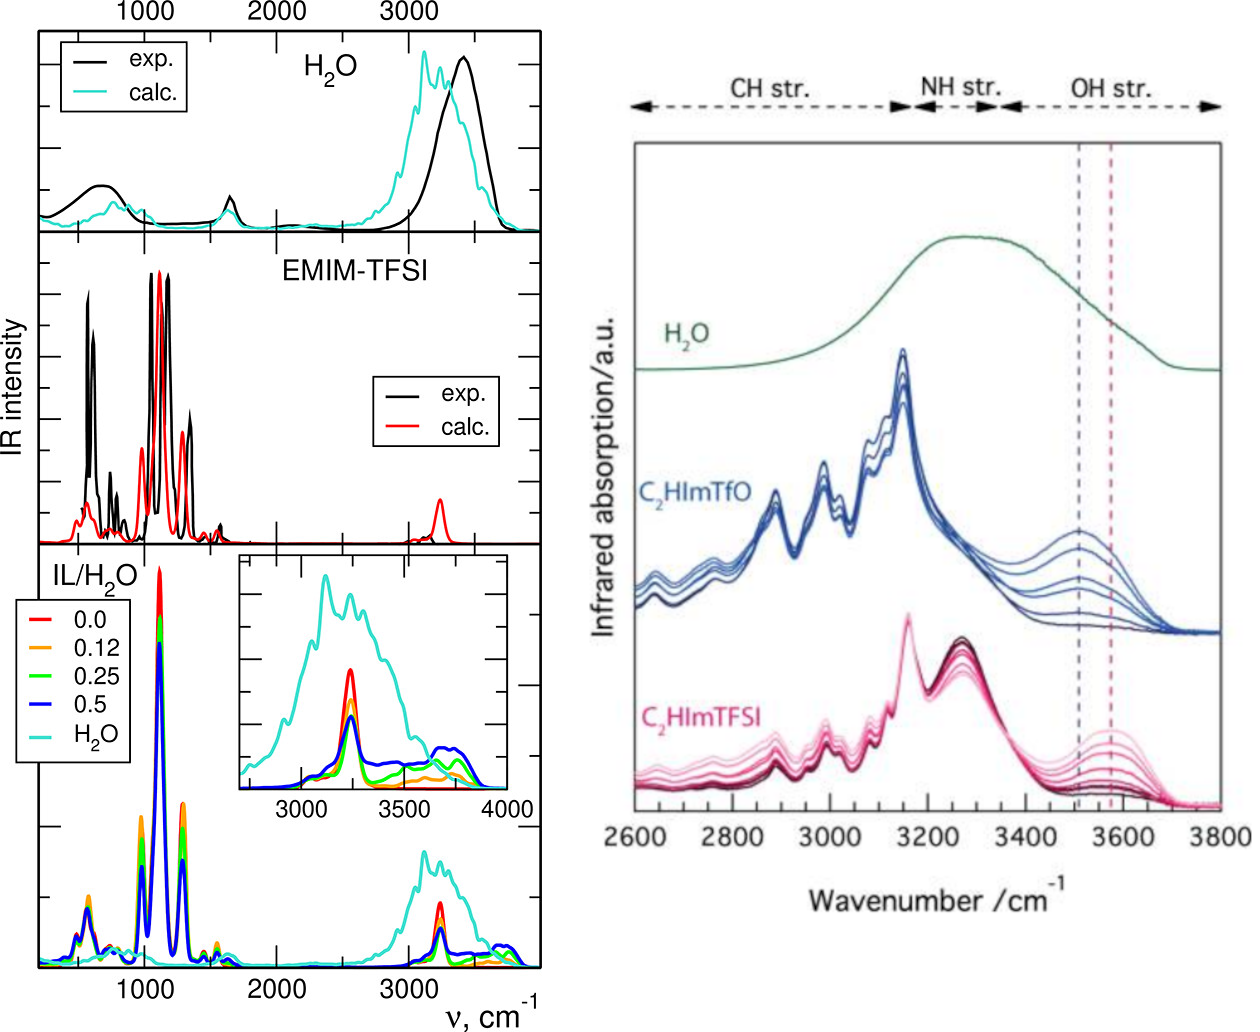
\includegraphics[width=0.75\textwidth]{img/4-ir-spectra-from-aimd-simulations/4-il-h2o/ir-spectra.png}
    \caption{IR spectra calculated from AIMD trajectories for neat liquids and IL/water mixtures with increasing mole fraction of water, experimental spectra are from~\cite{experimental-ir-h2o} for water and from~\cite{experimental-ir-emim-tfsi} for IL (left); experimental spectra for H$_2$O and IL/H$_2$O mixtures (right)~\cite{experimental-ir-emim-tfsi-h2o}, for EMIM-TFSI changes are shown in the bottom}
    \label{fig:il-h2o-ir-spectra}
\end{figure}

IR spectra are presented as averages over all replicas in Figure~\ref{fig:il-h2o-ir-spectra}. For comparison experimental spectra of water~\cite{experimental-ir-h2o}, EMIM-TFSI~\cite{experimental-ir-emim-tfsi} and IL/H$_2$O mixtures~\cite{experimental-ir-emim-tfsi-h2o} are shown.

There are some differences between calculated and experimental spectra of neat liquids. While computed frequencies of the H-O-H bending mode in water at 1600~cm$^{-1}$ agree with measured data, the O-H stretching band above 3000~cm$^{-1}$ is shifted by 200-250~cm$^{-1}$ to lower energies with respect to the experiment. For EMIM-TFSI, the shape of the spectrum is predicted correctly, but the part below 1500~cm$^{-1}$ is shifted to lower frequencies by about 60~cm$^{-1}$, the intensity of the band at 980~cm$^{-1}$ is too low and C-H stretching bands are shifted to higher energies. However, these results are similar to benchmarking tests of applying different functionals to liquid methanol~\cite{dft-methanol-benchmark}, so the differences with respect to measured spectra are considered as acceptable.

For mixtures, with growing amount of water the intensities of IL-related bands decrease due to decreasing concentration of ions in the solution. More significant changes are observed above 3000~cm$^{-1}$. At first, a~small increase of intensity below C-H band at 3240~cm$^{-1}$ is observed. It may be attributed to shifts of the C-H vibrations in EMIM$^{+}$ cations which are in an environment different than in the neat IL. The IR intensity between 3300 and 3800~cm$^{-1}$ increases with appearance of a~new maximum at about 3700-3750~cm$^{-1}$. This could be related to O-H vibrations in H$_2$O molecules. The new maximum is located above the main maximum observed for neat water, so the water molecules are apparently in different environment than in a~bulk water with smaller degree of water-water hydrogen bonding (what is confirmed by the analysis of structural data in section~\ref{section:il-h2o-structural}). Calculated changes agree with changes observed experimentally for EMIM-TFSI/H$_2$O~\cite{experimental-ir-emim-tfsi-h2o} (right panel of Figure~\ref{fig:il-h2o-ir-spectra}) and EMIM-BF$_4$-H$_2$O~\cite{experimental-ir-emim-bf4-h2o} mixtures.

\begin{figure}[ht]
    \centering
    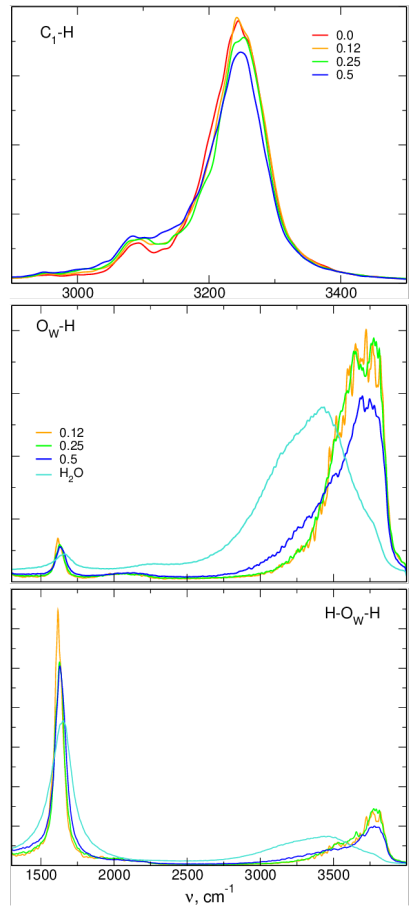
\includegraphics[width=0.4\textwidth]{img/4-ir-spectra-from-aimd-simulations/4-il-h2o/fourier-averages.png}
    \caption{Fourier transforms of C$_1$-H, O$_w$-H bond lengths and H-O$_w$-H angles averaged over all ions/molecules in IL/water mixtures}
    \label{fig:il-h2o-fourier-averages}
\end{figure}

As for previously described systems, Fourier transforms of selected geometrical parameters of the system were calculated to get a~deeper insight into interactions. Figure~\ref{fig:il-h2o-fourier-averages} shows FTs of C$_1$-H, O$_w$-H bond lengths and H-O$_w$-H angles averaged over all molecules/ions (labels of atoms are the same as in Figure~\ref{fig:il-h2o-emim-labeling}). Similar changes to those obtained for IR spectra in mentioned above ranges can be observed.

\begin{figure}[ht]
    \centering
    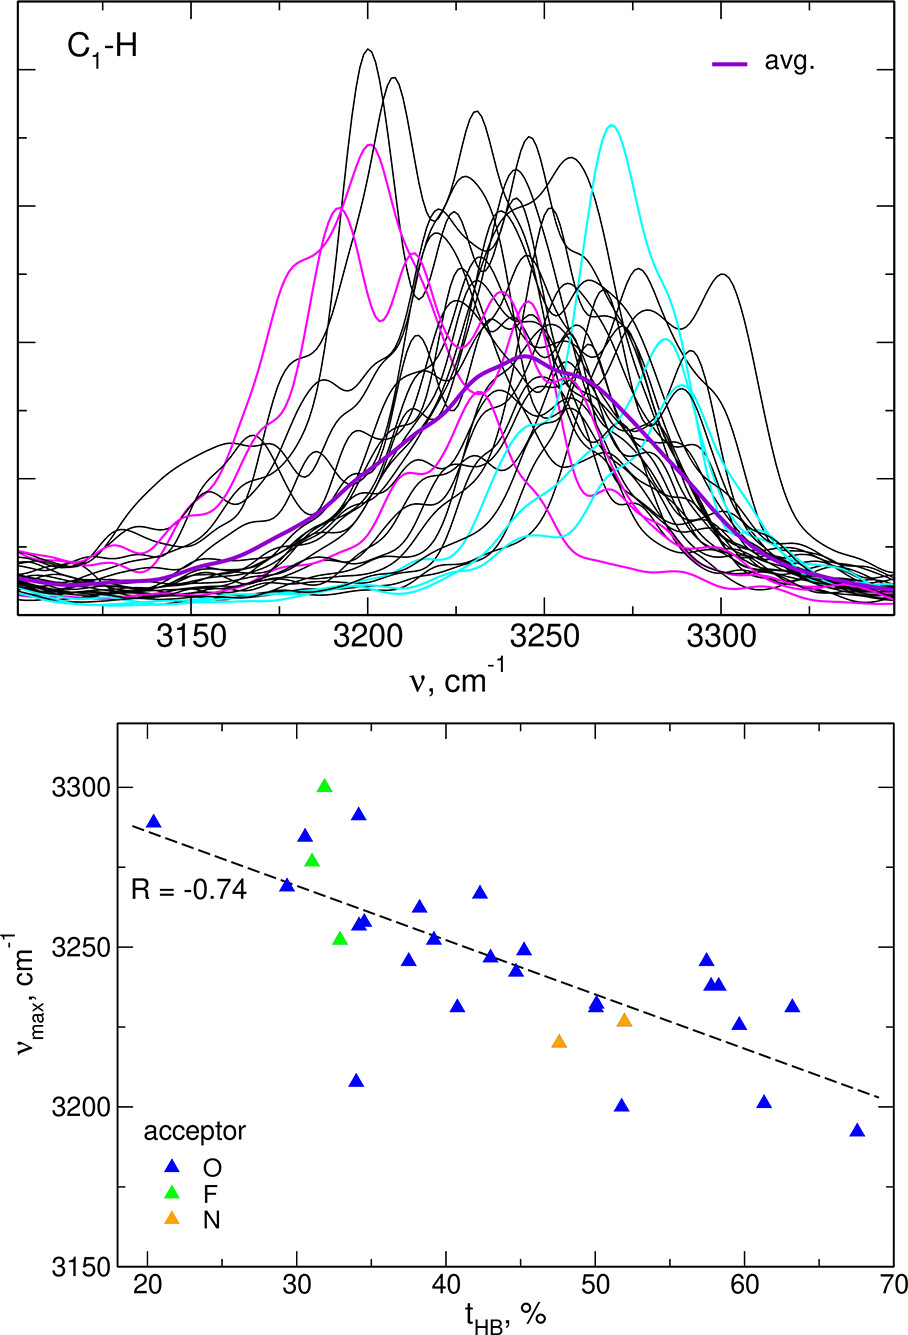
\includegraphics[width=0.4\textwidth]{img/4-ir-spectra-from-aimd-simulations/4-il-h2o/c-h-corr-0.png}
    \caption{Fourier transforms of C$_1$-H bond lengths in neat EMIM-TFSI (top), positions of maxima in FTs of bond lengths vs the time of HB formation (bottom)}
    \label{fig:il-h2o-c-h-corr-0}
\end{figure}

In Figure~\ref{fig:il-h2o-c-h-corr-0} individual Fourier transforms for all C$_1$-H bond lengths in neat EMIM-TFSI are presented. Positions of maxima vary in an interval of about 200~cm$^{-1}$ with an average at 3250~cm$^{-1}$ (purple line). Three EMIM$^{+}$ ions which spent most time forming HB from C$_1$-H group to TFSI$^{-}$ are shown in magenta and three ions with the shortest time of such HB formation are marked in cyan. It can be seen that, frequencies of C-H vibrations involved in HB formation are shifted below the average frequency while frequencies of "free" C-H bonds (with small times of HB formation) are shifted to higher values than average. It should be noted here, that these differences are the~result of different chemical environment of particular molecules during the limited simulation time and for a~sufficiently long trajectory, all of them would be on average in the same environment and differenes between FTs would be small.

The bottom panel of Figure~\ref{fig:il-h2o-c-h-corr-0} shows the plot of position of a~maximum of C$_1$-H FT vs average time spent on formation of HB. These two parameters are correlated, the longer is the time of HB existence the lower is the frequency of the C$_1$-H stretch. Majority of acceptors here are oxygen atoms, the size of the system did not allow to make a~reasonable analysis for different acceptors (O, F or~N). However, the plot suggests that changes for donors making HBs with fluorine acceptors are smaller than the others.

\begin{figure}[ht]
    \centering
    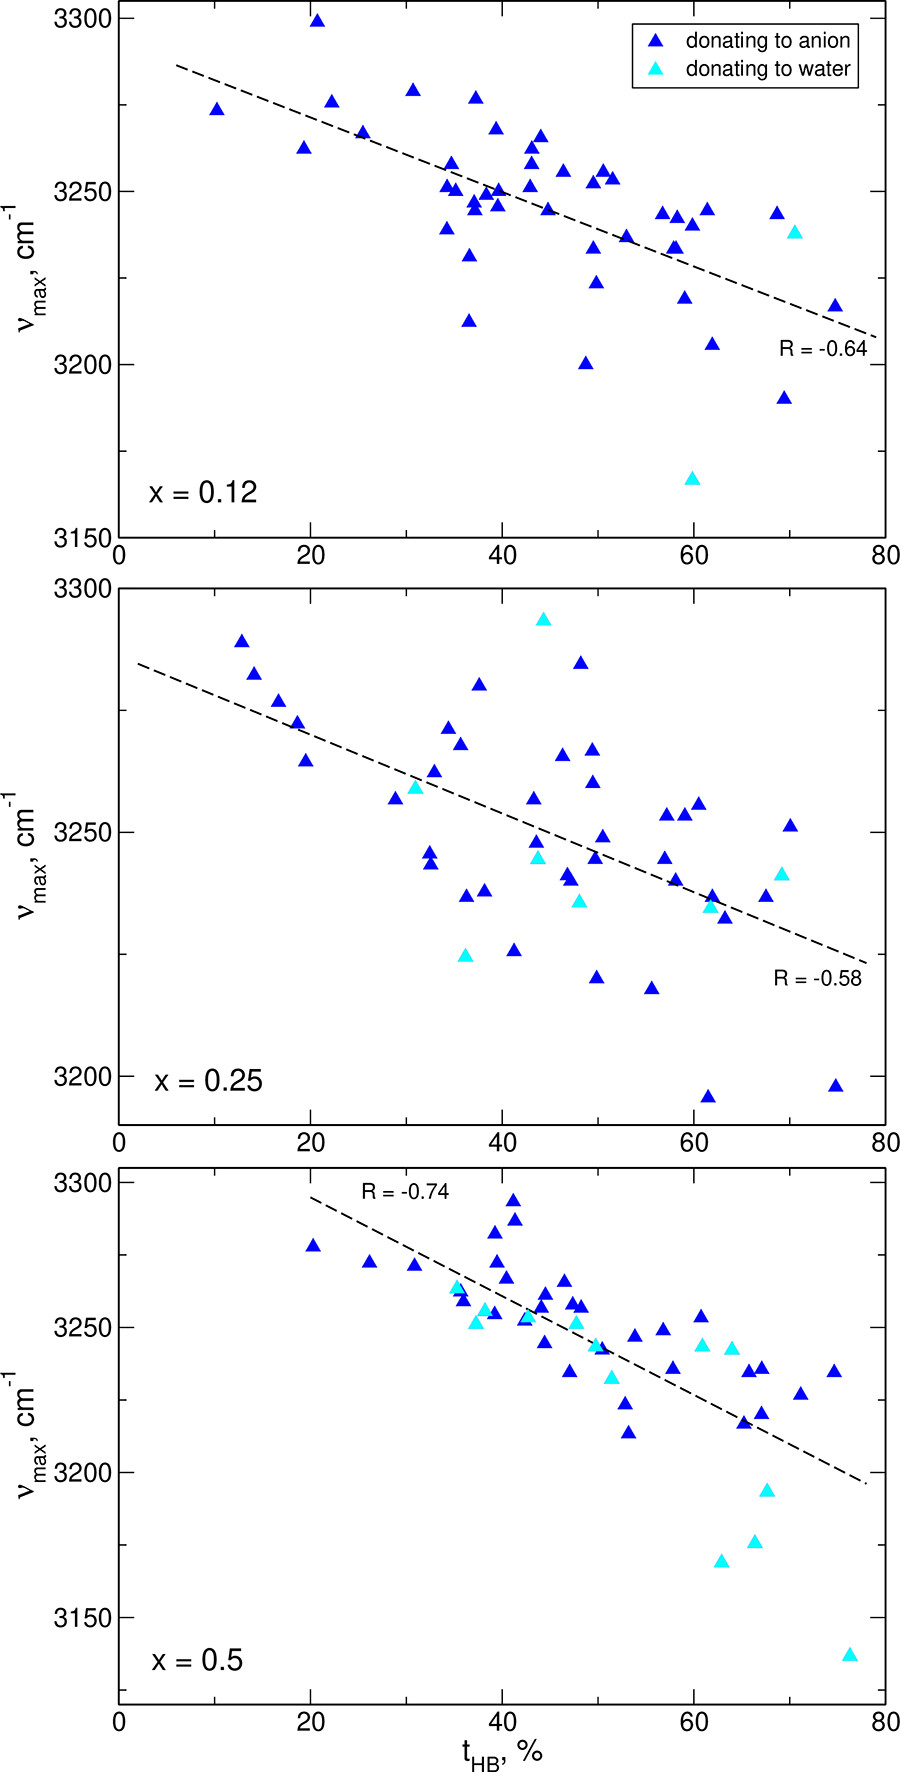
\includegraphics[width=0.4\textwidth]{img/4-ir-spectra-from-aimd-simulations/4-il-h2o/c-h-corr-mixtures.png}
    \caption{Positions of the maxima in FTs of C$_1$-H bond lengths vs the time of HB formation for IL/water mixtures}
    \label{fig:il-h2o-c-h-corr-mixtures}
\end{figure}

Similar analysis for systems containing water is presented in Figure~\ref{fig:il-h2o-c-h-corr-mixtures}. In all three systems, the observed correlation is similiar to this in neat IL: HB formation decreases the frequency of a~C$_1$-H vibration. There is no clear correlation with the type of acceptor (TFSI$^{-}$ or water), perhaps with the exception of the system with $x = 0.5$ where the most red-shifted vibrations engage water molecules. However, again the sizes of the systems in AIMD were too small to collect more detailed data and split it by the type of the acceptor.

Results from Figures~\ref{fig:il-h2o-c-h-corr-0} and~\ref{fig:il-h2o-c-h-corr-mixtures} confirm predictions about origins of changes observed in IR spectra. An increase of intensity observed below 3250~cm$^{-1}$ in water-containing samples is related to changes in HB formation of H~atoms from imidazolium ring of EMIM$^{+}$ cations. It is confirmed by statistics of increased probability of HB formation by imidazolium hydrogens with increasing water fraction (Figure~\ref{fig:il-h2o-hb-statistics}).

From experimental measurements of Raman spectra for water it is known that "free" (not being a~donor of a~HB) O-H bonds appear at the highest frequencies (about 3600~cm$^{-1}$). Frequencies of O-H vibrations in water molecules involved in HBs decrease in order DDA, DA, DDAA and DAA, depending on the HB configuration of a~given molecule. Here, D and A denote that the H$_2$O molecule serves as a~donor and acceptor of a~HB, respectively. For example, DDA configuration means that the molecule is an acceptor of one hydrogen atom from another molecule and simultaneously donates both hydrogen atoms to two other molecules. From deconvolution of Raman spectrum is was shown that the frequency of the DDAA configuration ("tetrahedral") is equal about 3200~cm$^{-1}$ and the other main contribution originates from DA configuration (about 3400~cm$^{-1}$)~\cite{h2o-bands-raman}.

\begin{figure}[ht]
    \centering
    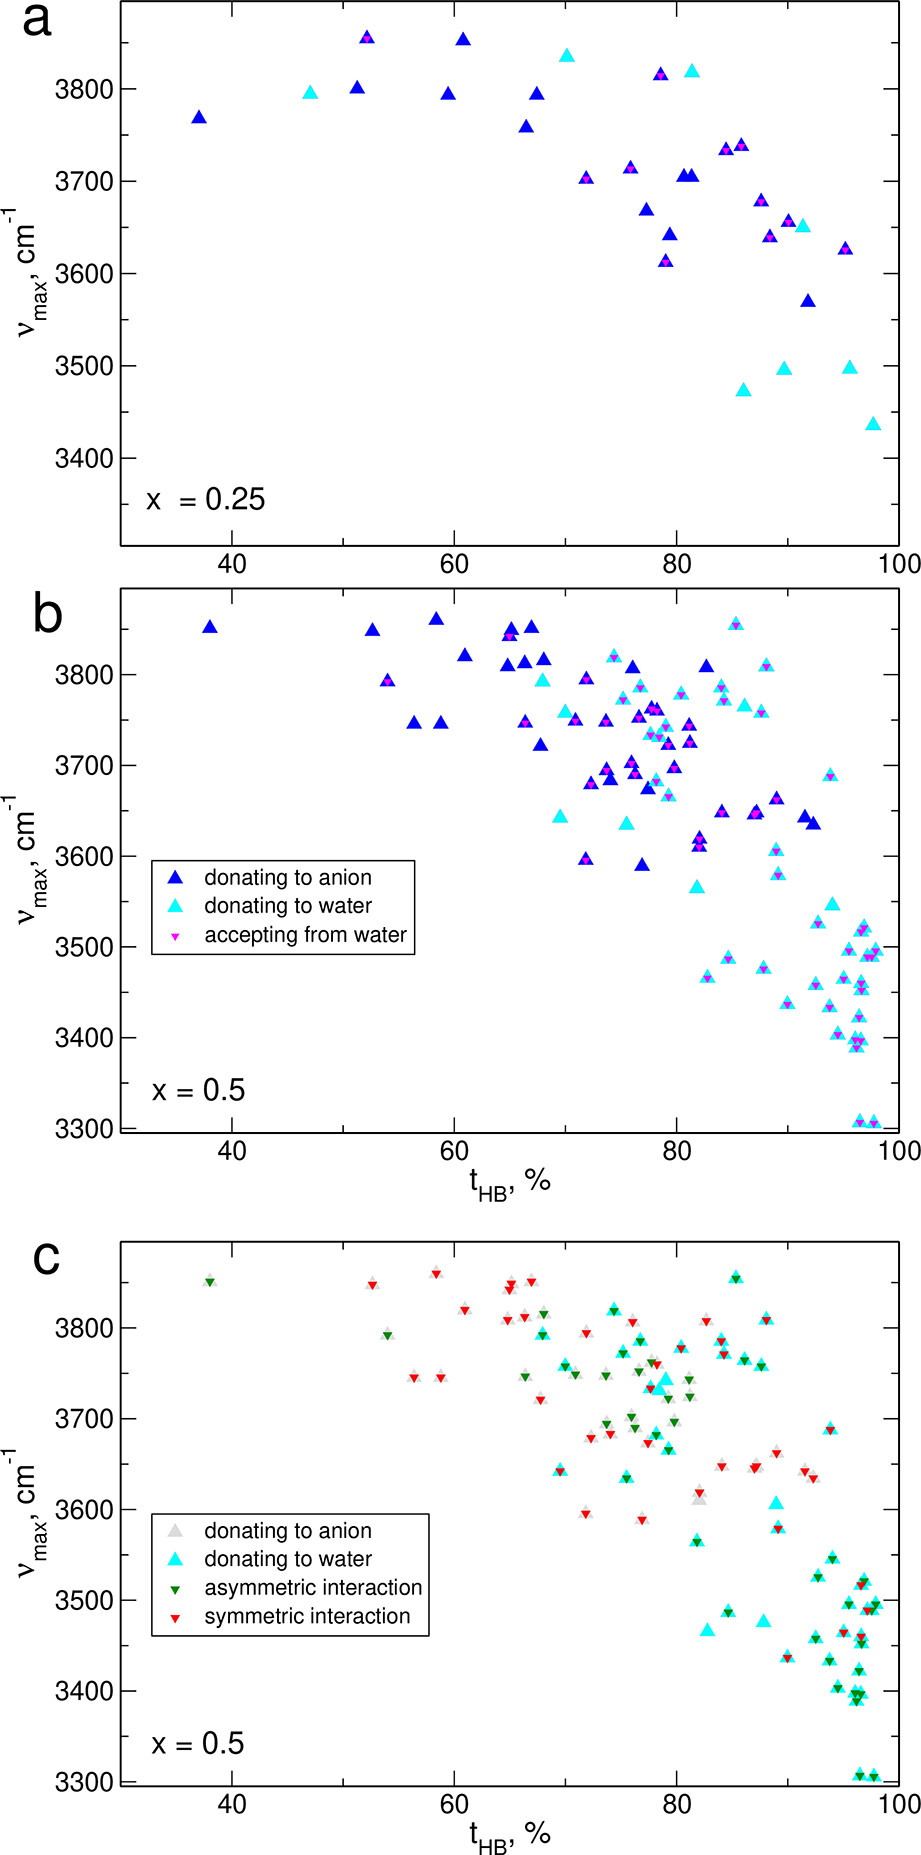
\includegraphics[width=0.4\textwidth]{img/4-ir-spectra-from-aimd-simulations/4-il-h2o/o-h-corr-mixtures.png}
    \caption{Positions of the maxima in FTs of O-H bond lengths vs the time of HB formation for IL/water mixtures with $x = 0.25$ (a), $x = 0.5$ (b) and with alternative labeling of data for $x = 0.5$ (c)}
    \label{fig:il-h2o-o-h-corr-mixtures}
\end{figure}

Figure~\ref{fig:il-h2o-o-h-corr-mixtures}a,b shows the dependence of O-H stretching frequency vs percentage of the time of HB formation for two systems with the highest water concentration. In general, the biggest the time of HB formation, the biggest red shift of related O-H stretching frequency is observed. It could be also noted, that the configuration of HBs for a~given molecule is also essential, donation of H~atom to TFSI$^{-}$ anion results in smaller red-shifts than the donation to water molecule, and the effect is even bigger when the H$_2$O molecule is also an acceptor of HB from another H$_2$O molecule. Thus, the lowest frequencies are observed for molecules with configurations which are the most close to those in bulk water - for H$_2$O molecules which are simultaneously H-acceptors and H-donors from/to other water molecules. However, in studied systems the number of such water molecules is limited. Some water molecules are involved only as H-donors to TFSI$^{-}$ anions, for them the O-H frequency is usually between 3850 and 3700~cm$^{-1}$. It is lowered to 3800-3600~cm$^{-1}$ when the water molecule donating to TFSI$^{-}$ anion becomes also an HB acceptor from another H$_2$O molecule. For molecules, which are not an acceptor of HB from water but are donors of HB to another water molecule, the frequency is in the range 3800-3500~cm$^{-1}$. All mentioned frequencies are higher than these for bulk water, what is a~result of the fact that in studied systems water molecules were in environment modified by the presence of the IL. Therefore, as it was seen in Figure~\ref{fig:il-h2o-ir-spectra}, a~new band with a~frequency above the O-H frequency for bulk water appears (at about 3700-3750~cm$^{-1}$).

Figure~\ref{fig:il-h2o-o-h-corr-mixtures}c shows an alternative labeling for data from the system with $x = 0.5$ in agreement with symmetry of the environment of two O-H bonds in the water molecule defined in~\cite{experimental-ir-emim-bf4-h2o}. Here, there is also a~color-coding of the distinction between symmetric hydrogen bonding (both O-H groups form HBs to the same type of acceptor for a~similar time) and asymmetric hydrogen bonding (the acceptors for two O-H bonds are different or there is a~substantial time difference of formation of HB for these bonds). According to~\cite{experimental-ir-emim-bf4-h2o}, frequencies of O-H stretch depend on this symmetry as follows: $\nu_{ab} < \nu_s < \nu_{af}$ where $\nu_s$ is the frequency in symmetric environment and $\nu_{ab}$ and $\nu_{af}$ are frequencies of either "bound" or "free" O-H groups in asymmetric configuration. Therefore, the lowest frequencies are computed for O-H bonds donating to water in an asymmetric environment. It could be expected that the highest frequencies would be observed for O-H groups interacting asymetrically with anion for short time. In studied $x = 0.5$ system only one such O-H vibration is visible, but still its frequency is among the highest calculated. So, the general trend from~\cite{experimental-ir-emim-bf4-h2o} is present in the shown data, however to be able to perform a~more detailed analysis one should perform longer simulations for larger systems to obtain better statistics.

\cleardoublepage